
%% bare_conf.tex
%% V1.3
%% 2007/01/11
%% by Michael Shell
%% See:
%% http://www.michaelshell.org/
%% for current contact information.
%%
%% This is a skeleton file demonstrating the use of IEEEtran.cls
%% (requires IEEEtran.cls version 1.7 or later) with an IEEE conference paper.
%%
%% Support sites:
%% http://www.michaelshell.org/tex/ieeetran/
%% http://www.ctan.org/tex-archive/macros/latex/contrib/IEEEtran/
%% and
%% http://www.ieee.org/

%%*************************************************************************
%% Legal Notice:
%% This code is offered as-is without any warranty either expressed or
%% implied; without even the implied warranty of MERCHANTABILITY or
%% FITNESS FOR A PARTICULAR PURPOSE! 
%% User assumes all risk.
%% In no event shall IEEE or any contributor to this code be liable for
%% any damages or losses, including, but not limited to, incidental,
%% consequential, or any other damages, resulting from the use or misuse
%% of any information contained here.
%%
%% All comments are the opinions of their respective authors and are not
%% necessarily endorsed by the IEEE.
%%
%% This work is distributed under the LaTeX Project Public License (LPPL)
%% ( http://www.latex-project.org/ ) version 1.3, and may be freely used,
%% distributed and modified. A copy of the LPPL, version 1.3, is included
%% in the base LaTeX documentation of all distributions of LaTeX released
%% 2003/12/01 or later.
%% Retain all contribution notices and credits.
%% ** Modified files should be clearly indicated as such, including  **
%% ** renaming them and changing author support contact information. **
%%
%% File list of work: IEEEtran.cls, IEEEtran_HOWTO.pdf, bare_adv.tex,
%%                    bare_conf.tex, bare_jrnl.tex, bare_jrnl_compsoc.tex
%%*************************************************************************

% *** Authors should verify (and, if needed, correct) their LaTeX system  ***
% *** with the testflow diagnostic prior to trusting their LaTeX platform ***
% *** with production work. IEEE's font choices can trigger bugs that do  ***
% *** not appear when using other class files.                            ***
% The testflow support page is at:
% http://www.michaelshell.org/tex/testflow/



% Note that the a4paper option is mainly intended so that authors in
% countries using A4 can easily print to A4 and see how their papers will
% look in print - the typesetting of the document will not typically be
% affected with changes in paper size (but the bottom and side margins will).
% Use the testflow package mentioned above to verify correct handling of
% both paper sizes by the user's LaTeX system.
%
% Also note that the "draftcls" or "draftclsnofoot", not "draft", option
% should be used if it is desired that the figures are to be displayed in
% draft mode.
%
\documentclass[a4paper, 12pt]{article}
\usepackage{fullpage}
% Add the compsoc option for Computer Society conferences.
%
% If IEEEtran.cls has not been installed into the LaTeX system files,
% manually specify the path to it like:
% \documentclass[conference]{../sty/IEEEtran}





% Some very useful LaTeX packages include:
% (uncomment the ones you want to load)


% *** MISC UTILITY PACKAGES ***
%
%\usepackage{ifpdf}
% Heiko Oberdiek's ifpdf.sty is very useful if you need conditional
% compilation based on whether the output is pdf or dvi.
% usage:
% \ifpdf
%   % pdf code
% \else
%   % dvi code
% \fi
% The latest version of ifpdf.sty can be obtained from:
% http://www.ctan.org/tex-archive/macros/latex/contrib/oberdiek/
% Also, note that IEEEtran.cls V1.7 and later provides a builtin
% \ifCLASSINFOpdf conditional that works the same way.
% When switching from latex to pdflatex and vice-versa, the compiler may
% have to be run twice to clear warning/error messages.






% *** CITATION PACKAGES ***
%
\usepackage{cite}
% cite.sty was written by Donald Arseneau
% V1.6 and later of IEEEtran pre-defines the format of the cite.sty package
% \cite{} output to follow that of IEEE. Loading the cite package will
% result in citation numbers being automatically sorted and properly
% "compressed/ranged". e.g., [1], [9], [2], [7], [5], [6] without using
% cite.sty will become [1], [2], [5]--[7], [9] using cite.sty. cite.sty's
% \cite will automatically add leading space, if needed. Use cite.sty's
% noadjust option (cite.sty V3.8 and later) if you want to turn this off.
% cite.sty is already installed on most LaTeX systems. Be sure and use
% version 4.0 (2003-05-27) and later if using hyperref.sty. cite.sty does
% not currently provide for hyperlinked citations.
% The latest version can be obtained at:
% http://www.ctan.org/tex-archive/macros/latex/contrib/cite/
% The documentation is contained in the cite.sty file itself.






% *** GRAPHICS RELATED PACKAGES ***
%
	\usepackage[pdftex]{graphicx}
  % declare the path(s) where your graphic files are
  % \graphicspath{{../pdf/}{../jpeg/}}
  % and their extensions so you won't have to specify these with
  % every instance of \includegraphics
  % \DeclareGraphicsExtensions{.pdf,.jpeg,.png}

  % or other class option (dvipsone, dvipdf, if not using dvips). graphicx
  % will default to the driver specified in the system graphics.cfg if no
  % driver is specified.
  % \usepackage[dvips]{graphicx}
  % declare the path(s) where your graphic files are
  % \graphicspath{{../eps/}}
  % and their extensions so you won't have to specify these with
  % every instance of \includegraphics
  % \DeclareGraphicsExtensions{.eps}

% graphicx was written by David Carlisle and Sebastian Rahtz. It is
% required if you want graphics, photos, etc. graphicx.sty is already
% installed on most LaTeX systems. The latest version and documentation can
% be obtained at: 
% http://www.ctan.org/tex-archive/macros/latex/required/graphics/
% Another good source of documentation is "Using Imported Graphics in
% LaTeX2e" by Keith Reckdahl which can be found as epslatex.ps or
% epslatex.pdf at: http://www.ctan.org/tex-archive/info/
%
% latex, and pdflatex in dvi mode, support graphics in encapsulated
% postscript (.eps) format. pdflatex in pdf mode supports graphics
% in .pdf, .jpeg, .png and .mps (metapost) formats. Users should ensure
% that all non-photo figures use a vector format (.eps, .pdf, .mps) and
% not a bitmapped formats (.jpeg, .png). IEEE frowns on bitmapped formats
% which can result in "jaggedy"/blurry rendering of lines and letters as
% well as large increases in file sizes.
%
% You can find documentation about the pdfTeX application at:
% http://www.tug.org/applications/pdftex





% *** MATH PACKAGES ***
%
\usepackage[cmex10]{amsmath}
% A popular package from the American Mathematical Society that provides
% many useful and powerful commands for dealing with mathematics. If using
% it, be sure to load this package with the cmex10 option to ensure that
% only type 1 fonts will utilized at all point sizes. Without this option,
% it is possible that some math symbols, particularly those within
% footnotes, will be rendered in bitmap form which will result in a
% document that can not be IEEE Xplore compliant!
%
% Also, note that the amsmath package sets \interdisplaylinepenalty to 10000
% thus preventing page breaks from occurring within multiline equations. Use:
%\interdisplaylinepenalty=2500
% after loading amsmath to restore such page breaks as IEEEtran.cls normally
% does. amsmath.sty is already installed on most LaTeX systems. The latest
% version and documentation can be obtained at:
% http://www.ctan.org/tex-archive/macros/latex/required/amslatex/math/





% *** SPECIALIZED LIST PACKAGES ***
%
%\usepackage{algorithmic}
% algorithmic.sty was written by Peter Williams and Rogerio Brito.
% This package provides an algorithmic environment fo describing algorithms.
% You can use the algorithmic environment in-text or within a figure
% environment to provide for a floating algorithm. Do NOT use the algorithm
% floating environment provided by algorithm.sty (by the same authors) or
% algorithm2e.sty (by Christophe Fiorio) as IEEE does not use dedicated
% algorithm float types and packages that provide these will not provide
% correct IEEE style captions. The latest version and documentation of
% algorithmic.sty can be obtained at:
% http://www.ctan.org/tex-archive/macros/latex/contrib/algorithms/
% There is also a support site at:
% http://algorithms.berlios.de/index.html
% Also of interest may be the (relatively newer and more customizable)
% algorithmicx.sty package by Szasz Janos:
% http://www.ctan.org/tex-archive/macros/latex/contrib/algorithmicx/




% *** ALIGNMENT PACKAGES ***
%
%\usepackage{array}
% Frank Mittelbach's and David Carlisle's array.sty patches and improves
% the standard LaTeX2e array and tabular environments to provide better
% appearance and additional user controls. As the default LaTeX2e table
% generation code is lacking to the point of almost being broken with
% respect to the quality of the end results, all users are strongly
% advised to use an enhanced (at the very least that provided by array.sty)
% set of table tools. array.sty is already installed on most systems. The
% latest version and documentation can be obtained at:
% http://www.ctan.org/tex-archive/macros/latex/required/tools/


%\usepackage{mdwmath}
%\usepackage{mdwtab}
% Also highly recommended is Mark Wooding's extremely powerful MDW tools,
% especially mdwmath.sty and mdwtab.sty which are used to format equations
% and tables, respectively. The MDWtools set is already installed on most
% LaTeX systems. The lastest version and documentation is available at:
% http://www.ctan.org/tex-archive/macros/latex/contrib/mdwtools/


% IEEEtran contains the IEEEeqnarray family of commands that can be used to
% generate multiline equations as well as matrices, tables, etc., of high
% quality.


%\usepackage{eqparbox}
% Also of notable interest is Scott Pakin's eqparbox package for creating
% (automatically sized) equal width boxes - aka "natural width parboxes".
% Available at:
% http://www.ctan.org/tex-archive/macros/latex/contrib/eqparbox/





% *** SUBFIGURE PACKAGES ***
%\usepackage[tight,footnotesize]{subfigure}
% subfigure.sty was written by Steven Douglas Cochran. This package makes it
% easy to put subfigures in your figures. e.g., "Figure 1a and 1b". For IEEE
% work, it is a good idea to load it with the tight package option to reduce
% the amount of white space around the subfigures. subfigure.sty is already
% installed on most LaTeX systems. The latest version and documentation can
% be obtained at:
% http://www.ctan.org/tex-archive/obsolete/macros/latex/contrib/subfigure/
% subfigure.sty has been superceeded by subfig.sty.



%\usepackage[caption=false]{caption}
%\usepackage[font=footnotesize]{subfig}
% subfig.sty, also written by Steven Douglas Cochran, is the modern
% replacement for subfigure.sty. However, subfig.sty requires and
% automatically loads Axel Sommerfeldt's caption.sty which will override
% IEEEtran.cls handling of captions and this will result in nonIEEE style
% figure/table captions. To prevent this problem, be sure and preload
% caption.sty with its "caption=false" package option. This is will preserve
% IEEEtran.cls handing of captions. Version 1.3 (2005/06/28) and later 
% (recommended due to many improvements over 1.2) of subfig.sty supports
% the caption=false option directly:
%\usepackage[caption=false,font=footnotesize]{subfig}
%
% The latest version and documentation can be obtained at:
% http://www.ctan.org/tex-archive/macros/latex/contrib/subfig/
% The latest version and documentation of caption.sty can be obtained at:
% http://www.ctan.org/tex-archive/macros/latex/contrib/caption/




% *** FLOAT PACKAGES ***
%
%\usepackage{fixltx2e}
% fixltx2e, the successor to the earlier fix2col.sty, was written by
% Frank Mittelbach and David Carlisle. This package corrects a few problems
% in the LaTeX2e kernel, the most notable of which is that in current
% LaTeX2e releases, the ordering of single and double column floats is not
% guaranteed to be preserved. Thus, an unpatched LaTeX2e can allow a
% single column figure to be placed prior to an earlier double column
% figure. The latest version and documentation can be found at:
% http://www.ctan.org/tex-archive/macros/latex/base/



%\usepackage{stfloats}
% stfloats.sty was written by Sigitas Tolusis. This package gives LaTeX2e
% the ability to do double column floats at the bottom of the page as well
% as the top. (e.g., "\begin{figure*}[!b]" is not normally possible in
% LaTeX2e). It also provides a command:
%\fnbelowfloat
% to enable the placement of footnotes below bottom floats (the standard
% LaTeX2e kernel puts them above bottom floats). This is an invasive package
% which rewrites many portions of the LaTeX2e float routines. It may not work
% with other packages that modify the LaTeX2e float routines. The latest
% version and documentation can be obtained at:
% http://www.ctan.org/tex-archive/macros/latex/contrib/sttools/
% Documentation is contained in the stfloats.sty comments as well as in the
% presfull.pdf file. Do not use the stfloats baselinefloat ability as IEEE
% does not allow \baselineskip to stretch. Authors submitting work to the
% IEEE should note that IEEE rarely uses double column equations and
% that authors should try to avoid such use. Do not be tempted to use the
% cuted.sty or midfloat.sty packages (also by Sigitas Tolusis) as IEEE does
% not format its papers in such ways.





% *** PDF, URL AND HYPERLINK PACKAGES ***
%
%\usepackage{url}
% url.sty was written by Donald Arseneau. It provides better support for
% handling and breaking URLs. url.sty is already installed on most LaTeX
% systems. The latest version can be obtained at:
% http://www.ctan.org/tex-archive/macros/latex/contrib/misc/
% Read the url.sty source comments for usage information. Basically,
% \url{my_url_here}.





% *** Do not adjust lengths that control margins, column widths, etc. ***
% *** Do not use packages that alter fonts (such as pslatex).         ***
% There should be no need to do such things with IEEEtran.cls V1.6 and later.
% (Unless specifically asked to do so by the journal or conference you plan
% to submit to, of course. )


% correct bad hyphenation here
\hyphenation{op-tical net-works semi-conduc-tor}


\begin{document}
%
% paper title
% can use linebreaks \\ within to get better formatting as desired
\title{Evolving Robocode Controllers through  Grammatical Evolution}
% author names and affiliations
% use a multiple column layout for up to three different
% affiliations

\author{Y6380396}

% conference papers do not typically use \thanks and this command
% is locked out in conference mode. If really needed, such as for
% the acknowledgment of grants, issue a \IEEEoverridecommandlockouts
% after \documentclass

% for over three affiliations, or if they all won't fit within the width
% of the page, use this alternative format:
% 
%\author{\IEEEauthorblockN{Michael Shell\IEEEauthorrefmark{1},
%Homer Simpson\IEEEauthorrefmark{2},
%James Kirk\IEEEauthorrefmark{3}, 
%Montgomery Scott\IEEEauthorrefmark{3} and
%Eldon Tyrell\IEEEauthorrefmark{4}}
%\IEEEauthorblockA{\IEEEauthorrefmark{1}School of Electrical and Computer Engineering\\
%Georgia Institute of Technology,
%Atlanta, Georgia 30332--0250\\ Email: see http://www.michaelshell.org/contact.html}
%\IEEEauthorblockA{\IEEEauthorrefmark{2}Twentieth Century Fox, Springfield, USA\\
%Email: homer@thesimpsons.com}
%\IEEEauthorblockA{\IEEEauthorrefmark{3}Starfleet Academy, San Francisco, California 96678-2391\\
%Telephone: (800) 555--1212, Fax: (888) 555--1212}
%\IEEEauthorblockA{\IEEEauthorrefmark{4}Tyrell Inc., 123 Replicant Street, Los Angeles, California 90210--4321}}




% use for special paper notices
%\IEEEspecialpapernotice{(Invited Paper)}




% make the title area
\maketitle


\begin{abstract}
This paper begins with a brief overview of evolutionary computation and an introduction to grammatical evolution. An evolutionary algorithm which implements grammatical evolution is then designed in order to evolve Robocode robots. This algorithm is then implemented to determine how modifying the grammar specified for grammatical evolution affects the produced robots, specifically to determine if these robots can successfully battle opponents which they have never encountered before.
\end{abstract}
% IEEEtran.cls defaults to using nonbold math in the Abstract.
% This preserves the distinction between vectors and scalars. However,
% if the conference you are submitting to favors bold math in the abstract,
% then you can use LaTeX's standard command \boldmath at the very start
% of the abstract to achieve this. Many IEEE journals/conferences frown on
% math in the abstract anyway.

% no keywords




% For peer review papers, you can put extra information on the cover
% page as needed:
% \ifCLASSOPTIONpeerreview
% \begin{center} \bfseries EDICS Category: 3-BBND \end{center}
% \fi
%
% For peerreview papers, this IEEEtran command inserts a page break and
% creates the second title. It will be ignored for other modes.




\section{Introduction}
Humans have been evolving for millions of years, in this time we have acquired many traits which have proved essential to our survival. These traits have appeared due to random mutations in our genetic code over millions of generations. Although the chance of an individual mutation occurring is extremely low, the sheer number of opportunities at which one can occur allows for a large numbers of mutations in a population over time. 

In addition to mutation, reproduction allows the gene pool to diversify, producing combinations of traits, which, when combined, lead to greater survival rates and a more successful species. These techniques have arisen in nature and are the cause of the vast numbers of species found on earth today, every one of these species evolved from a common ancestor. If it were possible to do so, each individual organism could have its lineage traced back to this common ancestor. It would then be possible to see the series of mutations and reproductions that caused that particular organism to be. 

Instead of the genome of an organism, imagine that the organism itself was a computer program which was capable of reproducing and mutating its code. Such a program could change itself to adapt to situations which it had no previous experience of, if it had sufficient feedback from the environment about how successful it currently was. However this solitary program has a problem, there is no way for it to produce large amounts of new code spontaneously. Mutations will provide small changes, but in order to create a program which adapts quickly new code is required. What if, instead of a single program, there were a population of programs instead? Programs could exchange code which could create new and more effective strategies. This set-up effectively copies real world evolution and implements it as an algorithm, which, with a few changes, can be used to solve problems where code is required.

The aim of this paper is to produce a robot controller for Robocode. Robocode is a video game, implemented in Java, in which tank like robots fight each other in a walled arena. It is possible for any number of robots to fight in a battle, which consists of a number of rounds. In order to win a round a robot must destroy all other robots or be the robot with the highest score after a time limit. Every Robocode robot has a controller, where a controller is Java code which controls the robots actions. Many attempts have been made to design robots which are fully autonomous and some have been successful. Despite this, crafting a general purpose robot that can compete against any opponent is not a trivial problem as there are a large number of strategies available that must be countered.

Crafting the robot controller code manually can result in robots which do well against strategies which have been considered by the designer, but creating a robot which can compete well against unknown opponents is a far more involved task. Using the set-up from earlier, in which code can mutate and be exchanged between programs it is possible to design an algorithm to evolve robot controllers for use against general opponents. 

\section{Evolutionary Algorithms}

Evolutionary Computation is a well established field and there are many ways of writing an Evolutionary Algorithm which are already well explored. In order to select which type of algorithm to use, it is first necessary to understand how evolutionary computation works in general. The basic principles of an evolutionary algorithm state that there must be an initial population of individuals. This population can be of any size but it is important to note that larger population sizes increase the processing power required by the algorithm but smaller populations are often less diverse. The selection of population size is an important factor to consider when designing an evolutionary algorithm. 

In order for an evolutionary algorithm to function, it is necessary to be able to compare individuals against each other. For this purpose, each individual of the population is assigned a fitness. Fitness values can be calculated in many different ways, but it must be possible to compare one fitness against another and determine which is better, though it is possible for two individuals to have equal fitness. Choosing a fitness function, a function which computes the fitness value for an individual, is not a trivial decision and must be carefully considered.

An evolutionary algorithm functions through successive iterations, at each iteration the algorithm will have a current population, and will select individuals from this population to advance to the next iteration. This is known as \textit{selection}. There are many ways to implement selection, including \cite{jebari_selection_2013}:

\begin{itemize}
\item Roulette Wheel Selection
\item Tournament Selection
\item Elitism
\end{itemize}

Roulette wheel selection works by effectively placing each individual in the current population onto a roulette wheel, where the area of the wheel according to that individual is proportional to their fitness. This causes each individual to be selected by the wheel at a rate of:
\begin{equation}
\frac{fitness}{population fitness}
\end{equation}

Clearly, any individual with high fitness will be selected at a higher probability than those with low fitness, however, it is still possible for an individual with low fitness to be selected. This allows for variation in the current population to be passed to the next, while still allowing for a greater overall fitness in the next iteration. 

Tournament selection functions similarly with respect to outcome, but is different in execution from roulette wheel selection. For tournament selection, individuals are picked at random (independent of their fitness function) from the current population and are entered into a tournament with other randomly selected individuals. The probability of an individual winning this tournament is proportional to its fitness, similar to the roulette wheel selection probability. Tournament selection provides lower fitness individuals a greater chance of being selected for the next generation.

Elitism is not a selection method in itself, but it exists to enhance other selection methods. Elitism allows a number of the fittest individuals a free pass into the next iteration. Elitism should be used only when the fittest solutions must be preserved in the next generation, for example, in problems where fit solutions are extremely difficult to find. 

After the population of the next iteration has been selected, it must be manipulated to introduce further diversity, as without this evolutionary algorithms would stagnate. This is accomplished through two different methods, mutation and crossover. Mutation is performed on all individuals chosen by selection and randomly changes part of the individual, such as a single line of code, with a chosen probability. Each part of the individual is susceptible to mutation and each is checked independently of all others. The mutation probability is chosen when the evolutionary algorithm is designed and should always be less than 1 to prevent all individuals from being completely overwritten.

Crossover allows traits to be exchanged between individuals and is performed on pairs of individuals. For each pair of individuals in the population crossover is performed with a probability, similar to mutation. At a high level, crossover effectively swaps information between individuals, leaving two new individuals with traits from each of the selected individuals from the previous population.

\section{Grammatical Evolution}

Having discussed how evolutionary algorithms function as a whole it is clear that something is missing, how are the individuals from each generation represented? Answering this question is not trivial and there is not a single correct answer. However, all evolutionary algorithms use the same basic principles in order to represent the information being manipulated. All GAs must have a way to represent data internally, this must allow for the features of the GA, as discussed earlier, to be applied to it easily. This is the \textit{genotype} of the algorithm and is usually a data structure within whatever programming language has been used to implement the GA.  It is important that we can extract meaningful data from individuals, which is impossible if they only exist within a data structure in a GA. For this reason it is necessary to be able to transform a genotype into the entity it represents, or the \textit{phenotype}. It is possible to measure a phenotype in order to determine its fitness, unlike a genotype. As a side note, the individual items contained within a genotype are called \textit{codons}.

For the purposes of this paper it is required that code is generated, which narrows the choice of representation significantly. `Cartesian Genetic Programming' (CGP), described in \cite{miller_cartesian_2000}, allows programs to be generated and manipulated through evolutionary algorithms and is a good choice for many programming languages. However, due to the nature of the representation in CGP it is required that all of the functions or methods of the target programming language must be able to accept any other function or method as an argument. Of course, this is not possible in Java as the language is strongly-typed. For example a method which an argument of type \textit{int} could not accept a \textit{String} in place of that argument.

Fortunately, another representation exists which does not exhibit this flaw. `Grammatical Evolution' (GE), described in \cite{ryan_grammatical_1998} represents the genotype as a list of numbers. Of course, it is very easy to perform the basic features of a GA on a simple list, making GE a very efficient way of performing evolutionary computation. However, it is also necessary to be able to transform this genotype into a phenotype, in this case, usable Java code. This is accomplished through the use of a \textit{grammar} which defines every possible valid code string. For example, a subsection of a grammar which defines the Java language would be:
\begin{equation} \label{eq:bexp}
<boolean> := <boolean\_expression>| true | false
\end{equation}

This subsection illustrates that it is possible for a \textit{boolean} to represent either a \textit{boolean expression} or either of the literals \textit{true} and \textit{false}. The non terminal \textit{boolean\_expression} can be expanded further as per the definition of the grammar however the terminals \textit{true} and \textit{false} cannot. However, it is still required that it is possible to transform our genotype, which is a list of numbers into this phenotype. In order to do this the genotype is read sequentially in order to expand each non-terminal in the grammar. For example, using the grammar given in equation \ref{eq:bexp}, \textit{boolean} requires expansion. To expand this, the number, \textit{n}, at the current index of the genotype is read and the grammar is expanded according to:
\begin{equation} \label{eq:mod}
n\ mod\ c
\end{equation}

Where \textit{c} is the number of available choices for expansion. If \textit{n = 224} in this example, then the terminal \textit{true} would be selected, as the result of equation \ref{eq:mod} is \textit{2}. Using this method of grammar expansion it is always possible to generate a valid phenotype from a genotype unless the end of the genotype is reached. In this case, it is possible to simply wrap around to the beginning of the genotype and continue expanding from the start. Unfortunately, due to the way programming languages are structured it is possible to generate a genotype which translates to an infinite sequence of expansions in the grammar, creating an invalid phenotype. For this reason it is usually necessary to implement a limit on the number of times wrapping around the genotype is permitted and mark any individuals that breach this limit as having the lowest possible fitness. Despite this limitation GE has been selected as the representation for this paper.

\section{Algorithm Design}

The main goal of this paper is to design a Robocode robot which competes well against new and unknown opponents. In order to accomplish this an algorithm to evolve robot code must be designed. The base for this algorithm will be the Wallace framework, a evolutionary algorithm framework developed at the University of York. Wallace provides a good base on which to evolve robots and has many of the basic functions of an evolutionary algorithm built in. 

\subsection{Grammar Design}
Wallace is capable of performing GE and in order to do so must be provided with a grammar.  The design of the grammar contributes a great deal to the overall performance of the final robot. As such this paper will aim to develop three separate grammars and measure their effectiveness at producing a viable robot. The first of these grammars will be simple, and will restrict code generated to the basic functions of a robot: the \textit{basic grammar}. The second grammar will contain more advanced robot functions but will limit where functions can be called: the \textit{advanced grammar}. The third grammar will include the addition of two variables to the robot, a \textit{boolean} and an \textit{int}: the \textit{variable grammar}.

Robocode robots are allowed to execute code in two different ways: through a \textit{run()} method which is executed in its own thread (known here as the \textit{run code}) and a set of methods which execute when certain a certain event occurs (known here as the \textit{reactive code}). All of the grammars have the same basic design with regards to these two code types, the \textit{run()} method always contains a \textit{while(true)} loop which causes any code generated there to be run constantly, whereas reactive code is executed only once per event. Any variables passed to reactive code in event objects will be available to code executed in that method.

Robots are permitted to perform actions in two ways: by calling an \textit{immediate} method, such as \textit{turnLeft()} such that the action executes immediately, or by calling a \textit{set} method, such as \textit{setTurnLeft()} which causes the action to be added to a list of actions to execute later. In order to run the actions that are added to this list the method \textit{execute()} must be called. This functionality has been specified as mandatory in all grammars, and is done at the end of the while loop in \textit{run()}.

The simple grammar restricts its robots to only set methods, such that it cannot perform reactive behaviour in reactive code as it is only possible for the robot to add actions to the execute list. This does not stop reactive methods from affecting the behaviour of the robot, it simply reduces the complexity of generated robots. Additionally, the simple grammar only implements a subset of the available methods for reactive code, and the method \textit{onScannedRobot()} is fixed to a call to \textit{fire(1)} which causes robots to fire at an enemy automatically, a useful trait. Simple robots can generate arbitrarily long code sequences in both run and reactive code, this includes if...else-statements, however their grammar is simple compared to both others. The intention of developing the simple grammar is to attempt to determine if restricting the search space affects the ability to generate a viable robot. 

The advanced grammar adds a large amount of functionality over the simple grammar and allows for much more complex robots. All reactive code methods are implemented and custom code can be evolved in all of them, except for \textit{onScannedRobot()} which has been modified to allow a value to be evolved for \textit{fire()} which adjusts the power at which bullets are fired. For the advanced grammar, it is no longer possible to generate set methods in reactive code. Though this may appear to simplify the grammar it is countered by the addition of all possible immediate methods in reactive code. This allows the robot to react immediately to any event and means event code operates completely separately to run code. The most dramatic change between the advanced grammar and the simple grammar is the restriction on when certain actions can be executed and on when certain variables are accessible. The grammar has been modified so that the actions and variables in each reactive code method are a subset of all available methods, those that are more likely to be useful to the robot in that method. The aim of this change is to force the evolutionary algorithm to choose actions that are more realistic in the context of that method. For example, actions in the \textit{onHitWall()} method are restricted to those which cause movement, as attempting to shoot an opponent is pointless if you're running into a wall! The advanced grammar also includes the addition of the ability to generate simple if-statements in addition to if...else-statements. This change allows for more variation in the flow of control for all methods. 

The variable grammar, in addition to all advanced grammar functionality, adds the ability to get and set two private class variables, one \textit{boolean} and one \textit{int}. These variables are accessible from all methods and can be used in boolean expressions where appropriate. The intention of designing the variable grammar is to determine if robots can evolve complex stateful behaviour. The addition of this functionality dramatically increases the search space over which the solutions exist, and it is possible that the algorithm will not be able to find a good solution.

Creating these three grammars allows for an investigation into how changing the grammar affects robots produced though an evolutionary algorithm.

\subsection{Fitness Function}

Robocode battles provide many different metrics with which to quantify a robot, however not all of them are useful. Among the provided metrics are\cite{robocode_scoring}: 
\begin{itemize}
\item Score
\item Survival
\item Bullet Damage
\item First Places
\end{itemize}
At first glance, it would seem appropriate to simply take the robots score as its fitness. This is a valid choice, however the subtleties of how Robocode operates detracts from its appeal. Robots gain score based on how much they hit other robots, how well they dodge other robots bullets and gain bonus points for landing the killing shot on other robots \cite{robocode_scoring}. Using score alone for a fitness function presents a problem, it is not transferable between battles. For example, take two Robocode battles, one in which the score is 1500 to 500 and another in which the score is 2500 to 2500. In the first battle, the first robot would be evaluated with fitness 1500 and the second fitness 500. This is fair, the robot with the higher fitness is better. In the second battle, both robots would be evaluated with fitness 2500, this is also fair. However, if we were to use these fitnesses to compare the first robot from each battle, we would see that the robot from battle two is the fitter individual. This is surely not the case? The robot from battle one accumulated three times the score of its opponent and yet is worse than the robot from battle two! Score has clearly proven itself to be an inappropriate fitness function.

Unfortunately, none of the metrics available directly from Robocode are suitable for use as a fitness function directly. Survival does not take into account damage done to opponents, bullet damage does not account for robots that avoid bullets well and first places penalises robots which lose battles by a narrow margin. Fortunately, there is a simple way to modify score so that it can be used as a fitness function. If, instead of raw score, the robots percentage share of the total score is taken, then it is possible to evaluate how well a robot performed relative to the other robot in the battle. Using this metric, robots that narrowly lose battles are not punished and all aspects of performance are taken into account. This metric will be known as \textit{score share} and will be used for measuring robot fitness in this paper.

Score share allows for a robots performance in a single battle to be evaluated, however Robocode only permits a robot to fight one robot per battle for a fixed number of rounds. In order to evolve a robust solution, one which is capable of performing well against any opponent, a robot must battle many different opponents. A possible solution to this, is to battle against a specific opponent for a number of iterations, then change this opponent and repeat for any number of opponents. However, changing the robot battled during the algorithms execution effectively modifies the fitness function mid-run, which modifies the search landscape, effectively beginning the algorithm again at each opponent change. This `moving-target' algorithm would not be suitable for evolving Robocode robots as behaviours useful against early opponents could be overwritten later in the algorithm. 

If, instead of modifying the opponent robot during the algorithm, the opponent was kept constant this would allow the search space to be more effectively explored. Fortunately, our definition of fitness supports this option. As the chosen fitness function can only take values between 0 and 100 it is possible to obtain the mean score of a robot over multiple battles. If, at each evaluation of fitness, a robot fights a set of battles against different opponents and the mean fitness across all of these battles is calculated, the fitness function would reward general strategies which do well in all battles. Using this type of fitness function relies of having a good selection of opponents to face. Fortunately, Robocode is supplied with pre-built tanks which are designed to showcase different functionalities of the game, and they all use varying strategies! With this in mind, five robots were selected from the supplied Robocode sample robots for use: \textit{Fire}, \textit{TrackFire}, \textit{Tracker}, \textit{RamFire} and \textit{Walls}.

The chosen fitness function for this paper is the mean result of the score share from battles against the five chosen opponents, where each battle consists of five rounds. 

\subsection{Selection}

Wallace offers the following selection types: \textit{random}, \textit{roulette} and, \textit{tournament}. It is possible to add functionality to Wallace in order to support further types, however the three that already exist provide enough variation in functionality and were considered for use in this paper. 

Random selection, while not discussed previously, is a possible option for an evolutionary algorithm. This type of selection, however, offers no bias to high-fitness solutions and should be used with care. If random selection were to be used then elitism would almost certainly be required, guaranteeing the highest fitness individuals a place in the next iteration and then filling the rest of the population with randomly chosen individuals. Unfortunately, while providing an easy way to generate a diverse population quickly, random selection requires elitism, which reduces the diversity of the population in itself, making it a poor choice for this type of algorithm.

Roulette wheel selection provides a robust method of selection which favours fit individuals, however, unfit individuals are extremely unlikely to be chosen through this type of selection, causing the population to stagnate at high fitnesses. As this implementation will utilise Grammatical Evolution, individuals of all fitness levels are required in the population at all times. This is due to the possibility of an unfit solution receiving a mutation which completely changes its behaviour, improving its fitness dramatically. If every individual is similar then this is unlikely to occur and the population will stagnate. 

Tournament selection is, again, a robust method of selection, however, unlike roulette wheel selection, it favours unfit solutions slightly more. As the individuals which compete in tournaments are selected uniformly randomly from the population any set of individuals can be chosen, including those with low fitnesses. Of course, it is unlikely for an individual of low fitness to win the tournament, but, this is more likely than a low fitness individual being chosen by roulette wheel selection.

Tournament selection provides the best option for this algorithm as it does not eliminate low fitness solutions as easily as roulette wheel selection and provides a suitable bias to high fitness solutions simultaneously.

\subsection{Mutation}
When selecting how to apply mutation to a Grammatical Evolution it is important to understand what the genotype actually represents. Many types of mutation operate on binary phenotypes only and cannot be used for GE. Two interesting non-binary mutation types are: Gaussian Mutation and Uniform Mutation. 

Gaussian Mutation, instead of randomly mutating a chosen codon, adds a Gaussian random variable to the current value of the codon. This form of mutation is primarily used for genotypes that translate directly as numeric values in the phenotype. For GE, each codon represents a decision made when expanding a grammar, not a numeric value. Using Gaussian Mutation with a GE would not provide its intended effect, which is to localise the new codon value around that of the old. Nearness has no meaning when applied to a grammar derivation.

Uniform mutation is very simple, it simply uniformly randomly selects a new codon value to replace the old value. This is exactly what is required for use with GE, as the values have no numerical significance and are only used for the grammar derivation.

Uniform mutation was chosen for this paper.

\subsection{Crossover}
For the selection of crossover types there were three major competitors: one-point crossover, two-point crossover and uniform crossover. Again, choosing a crossover type requires understanding of the genotype and what it represents, as crossover manipulates many codons on each selected individuals genotype.

Both one and two-point crossover operate in a similar fashion, they both allow the exchange of codons between individuals,  however they are subtly different. One-point crossover picks a single point on the genotype for two individuals and swaps all codons after this point between those individuals. After the process two new individuals are produced. Two-point crossover works similarly, however instead of selecting a single point on both genotypes two points are selected, and the codons between these points are swapped. As it breaks the codons apart at two points, two-point crossover is more likely to break up codon chains which produce code with beneficial functions. Crossover is required for any evolutionary algorithm, but for GE it is necessary to break up codons as little as possible.

Uniform crossover works differently to both one and two-point crossover, in that instead of picking points on the genotype, it simply randomly shuffles the codons between both genotypes. This is extremely unsuitable for use with GE as codon chains which produce beneficial code will almost certainly be broken up on every single application of crossover. 

One-point crossover was selected for this paper as it preserves codon sequences but still provides variation in the population.


\subsection{Parameters}
As this paper aims to test the effectiveness of varying the grammar used for code generation there is little scope for the experimental determination of algorithm parameters, however informal testing was performed which led to the values used.

The crossover rate of the algorithm was set to 0.4; crossover rates that were too low failed to produce any variation in the population, whereas rates that were too high destroyed individuals which had high fitness too often. The mutation rate of the algorithm was set to 0.2; mutation can very easily turn a high fitness individual into a low fitness one with a single application, however if mutation rates are set too low then no variation can be generated in the population.

\section{Results}
In order to determine if the chosen grammar has an effect on the Robocode robots produced through evolutionary algorithms it is necessary to formulate a hypothesis to attempt to prove. Using the simple grammar as a base, formulating a hypothesis which claims that either the advanced or variable grammars produce robots which perform better than the simple grammar would cover this claim. Therefore the chosen hypothesis is: \textit{providing the given GE algorithm with a grammar which is more likely to result in Robocode controllers that have specific behaviours produces robots which perform better against new opponents}.
\begin{figure}[!t]
\centering
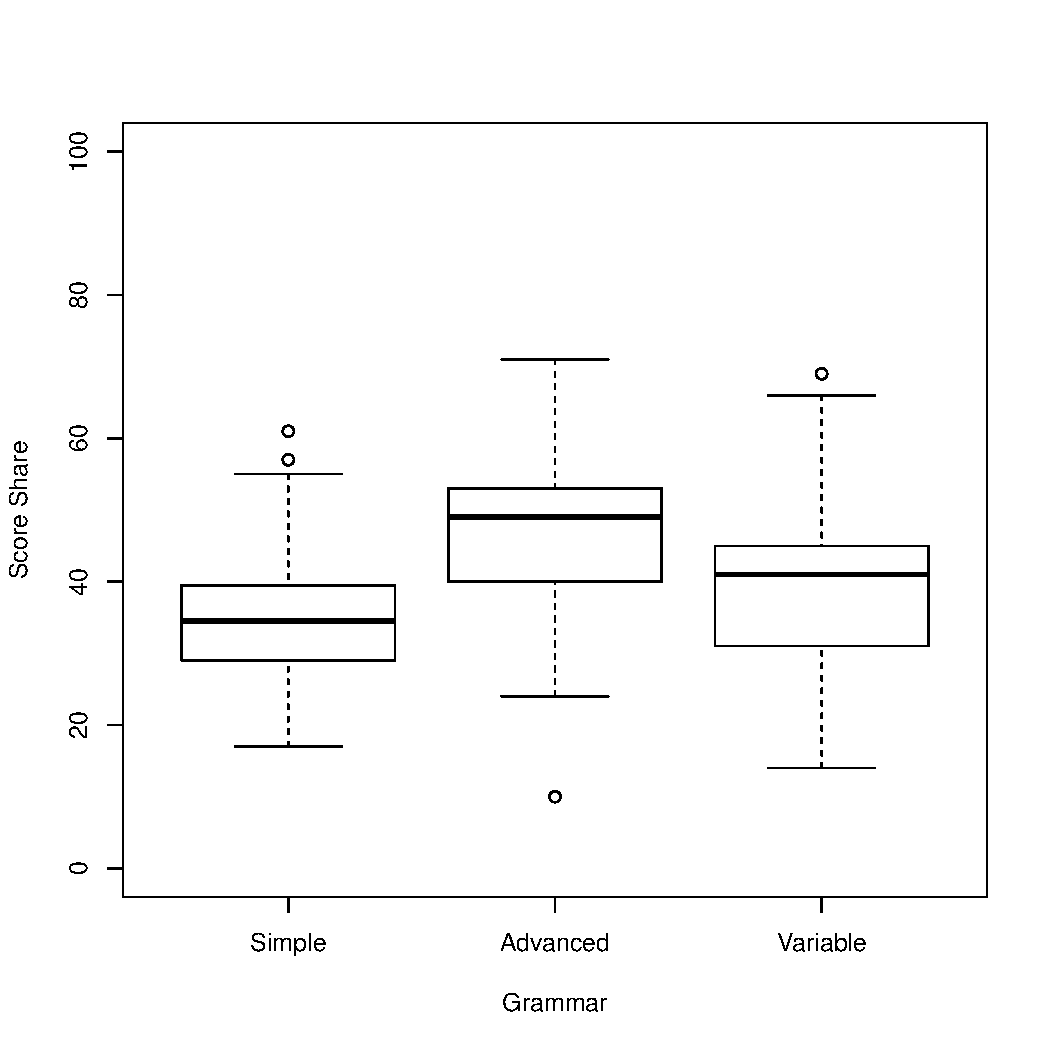
\includegraphics[width=4.5in]{figures/grammar_comparison.pdf}
\caption{Comparison of Grammar Performance}
\label{comp_plots}
\end{figure}
In order to test this claim, the GE algorithm was executed 10 times for each grammar. Each execution was limited to 500 evaluations, where an evaluation is one single call to the fitness function. In each case the individual with the highest fitness over all runs was selected and chosen as the \textit{representative} for that grammar. Then, in order to determine how well each grammar performed these representative robots battled a robot which was not used in the fitness function of the algorithm: \textit{VelociRobot}. This battle was repeated 100 times with 5 rounds per battle for each grammar representative in order to collect results which are statistically valid. Figure \ref{comp_plots} shows the results of these battles. 

It is difficult to tell if either the advanced or variable grammars perform better using figure \ref{comp_plots}. At first glance, it would appear as though both advanced and variable grammars produce robots which perform better than simple.  Indeed, upon close inspection it appears that the means for the advanced and variable grammars are greater than the mean for simple, but the spread of the data is somewhat large, preventing any useful conclusions from being drawn.

By using a statistical test to determine the differences between the data it is possible to gain further understanding into the differences between the data sets. As the data is non-parametric the Vargha and Delaney A measure can be used to determine if one data set is statistically significantly different to another. Performing this test between the data collected for advanced and simple yields a value of A = 0.7919. Though this shows that it is more likely for the advanced representative to produce a better result in a single battle than the simple representative, it is not possible to state with 95\% confidence that this is the case. A similar result is found for performing the same test between the data for variable and simple, yielding A = 0.63555, another statistically insignificant result.

As both sets of results are insignificant it is not possible to accept the hypothesis stated previously, but it is necessary to assume the null hypothesis: \textit{providing the given GE algorithm with a grammar which is more likely to result in Robocode controllers that have specific behaviours produces robots which perform no differently against new opponents}.


All statistical tests and plots were generated in R \cite{r_stats}.
\section{Conclusion}
Though this paper was unable to find any statistically significant results, this line of investigation with regard to grammar design is a valid aspect of evolutionary computation to explore. The way in which the grammars were designed for this paper was not particularly structured. Future work may wish to consider quantifying the complexity of grammars allowing for easier and more comprehensive analysis of performances between them.

Very little experimentation was performed in this paper with regard to the chosen parameters of the evolutionary algorithm features chosen. It may be possible that these parameters have subtle effects on the robots generated and this certainly warrants investigation. It is often somewhat difficult to evaluate these parameters as there are a very large number of viable combinations which produce operable algorithms. 

In addition to experimentation over which operating parameters are varied, it is possible to evaluate different choices of evolutionary algorithm features. This was not performed for this paper due to issues of scope, it is often difficult to effectively evaluate evolutionary algorithms as there are many possible configurations to be evaluated. Research into providing a means to test and compare evolutionary algorithms with different features would definitely be beneficial.

Finally, I personally found using evolutionary algorithms to evolve code extremely interesting, especially as this code was a controller for a game. Though the topic is well studied, I feel that there is always need for research into applying evolutionary algorithms to games, as they are often where great leaps forward are made, especially in the field of artificial intelligence. It would certainly be an amazing experience to have a conversation with an artificial intelligence constructed using an evolutionary algorithm!





% An example of a floating figure using the graphicx package.
% Note that \label must occur AFTER (or within) \caption.
% For figures, \caption should occur after the \includegraphics.
% Note that IEEEtran v1.7 and later has special internal code that
% is designed to preserve the operation of \label within \caption
% even when the captionsoff option is in effect. However, because
% of issues like this, it may be the safest practice to put all your
% \label just after \caption rather than within \caption{}.
%
% Reminder: the "draftcls" or "draftclsnofoot", not "draft", class
% option should be used if it is desired that the figures are to be
% displayed while in draft mode.
%
%\begin{figure}[!t]
%\centering
%\includegraphics[width=2.5in]{myfigure}
% where an .eps filename suffix will be assumed under latex, 
% and a .pdf suffix will be assumed for pdflatex; or what has been declared
% via \DeclareGraphicsExtensions.
%\caption{Simulation Results}
%\label{fig_sim}
%\end{figure}

% Note that IEEE typically puts floats only at the top, even when this
% results in a large percentage of a column being occupied by floats.


% An example of a double column floating figure using two subfigures.
% (The subfig.sty package must be loaded for this to work.)
% The subfigure \label commands are set within each subfloat command, the
% \label for the overall figure must come after \caption.
% \hfil must be used as a separator to get equal spacing.
% The subfigure.sty package works much the same way, except \subfigure is
% used instead of \subfloat.
%
%\begin{figure*}[!t]
%\centerline{\subfloat[Case I]\includegraphics[width=2.5in]{subfigcase1}%
%\label{fig_first_case}}
%\hfil
%\subfloat[Case II]{\includegraphics[width=2.5in]{subfigcase2}%
%\label{fig_second_case}}}
%\caption{Simulation results}
%\label{fig_sim}
%\end{figure*}
%
% Note that often IEEE papers with subfigures do not employ subfigure
% captions (using the optional argument to \subfloat), but instead will
% reference/describe all of them (a), (b), etc., within the main caption.


% An example of a floating table. Note that, for IEEE style tables, the 
% \caption command should come BEFORE the table. Table text will default to
% \footnotesize as IEEE normally uses this smaller font for tables.
% The \label must come after \caption as always.
%
%\begin{table}[!t]
%% increase table row spacing, adjust to taste
%\renewcommand{\arraystretch}{1.3}
% if using array.sty, it might be a good idea to tweak the value of
% \extrarowheight as needed to properly center the text within the cells
%\caption{An Example of a Table}
%\label{table_example}
%\centering
%% Some packages, such as MDW tools, offer better commands for making tables
%% than the plain LaTeX2e tabular which is used here.
%\begin{tabular}{|c||c|}
%\hline
%One & Two\\
%\hline
%Three & Four\\
%\hline
%\end{tabular}
%\end{table}


% Note that IEEE does not put floats in the very first column - or typically
% anywhere on the first page for that matter. Also, in-text middle ("here")
% positioning is not used. Most IEEE journals/conferences use top floats
% exclusively. Note that, LaTeX2e, unlike IEEE journals/conferences, places
% footnotes above bottom floats. This can be corrected via the \fnbelowfloat
% command of the stfloats package.




% conference papers do not normally have an appendix


% trigger a \newpage just before the given reference
% number - used to balance the columns on the last page
% adjust value as needed - may need to be readjusted if
% the document is modified later
%\IEEEtriggeratref{8}
% The "triggered" command can be changed if desired:
%\IEEEtriggercmd{\enlargethispage{-5in}}

% references section

% can use a bibliography generated by BibTeX as a .bbl file
% BibTeX documentation can be easily obtained at:
% http://www.ctan.org/tex-archive/biblio/bibtex/contrib/doc/
% The IEEEtran BibTeX style support page is at:
% http://www.michaelshell.org/tex/ieeetran/bibtex/
%\bibliographystyle{IEEEtran}
% argument is your BibTeX string definitions and bibliography database(s)
%\bibliography{IEEEabrv,../bib/paper}
%
% <OR> manually copy in the resultant .bbl file
% set second argument of \begin to the number of references
% (used to reserve space for the reference number labels box)

\bibliographystyle{IEEEtran}
\bibliography{IEEEabrv,evco_doc}





% that's all folks
\end{document}


